% e2m2e White Paper (English version)
% Build: xelatex (recommended: latexmk -xelatex main-en.tex)
\documentclass[11pt]{article}

\usepackage[T1]{fontenc}
\usepackage{lmodern}

\newcommand{\eEmTitle}{e2m2e White Paper}
\newcommand{\eEmVersion}{v5.8.8 \quad August 2026}

% e2m2e 白皮书共享导言区 / Shared preamble for the e2m2e white paper
% 语言相关的字体设置在各自的 main 文件中完成。
% Language-specific font setup lives in each main file.

\usepackage[a4paper,top=2.6cm,bottom=2.8cm,left=2.6cm,right=2.6cm]{geometry}
\usepackage{amsmath,amssymb,mathtools,bm}
\usepackage{graphicx}
\usepackage{xcolor}
\usepackage{booktabs,array,multirow,tabularx}
\usepackage{enumitem}
\usepackage{caption}
\usepackage{titlesec}
\usepackage{fancyhdr}
\usepackage{microtype}
\usepackage{tikz}
\usetikzlibrary{arrows.meta,positioning,shapes.geometric,fit,backgrounds,calc}
\usepackage[most]{tcolorbox}
\usepackage{listings}
\usepackage{hyperref}

% ---------------------------------------------------------------- 配色
\definecolor{e2blue}{HTML}{1B4F8A}   % 主色：深航天蓝
\definecolor{e2light}{HTML}{E8F0F8}  % 浅蓝底
\definecolor{e2gray}{HTML}{5A6570}
\definecolor{codebg}{HTML}{F5F7FA}
\definecolor{codeframe}{HTML}{D5DDE6}

\hypersetup{
  colorlinks=true,
  linkcolor=e2blue,
  urlcolor=e2blue,
  citecolor=e2blue,
  pdftitle={e2m2e White Paper},
  pdfauthor={cislunarspace},
}

% ---------------------------------------------------------------- 标题样式
\titleformat{\section}
  {\Large\bfseries\color{e2blue}}{\thesection}{0.8em}{}
  [{\color{e2blue}\titlerule[0.6pt]}]
\titleformat{\subsection}
  {\large\bfseries\color{e2blue!85!black}}{\thesubsection}{0.7em}{}
\titleformat{\subsubsection}
  {\normalsize\bfseries\color{e2gray}}{\thesubsubsection}{0.6em}{}
\titlespacing*{\section}{0pt}{2.2ex plus 1ex}{1.4ex}
\titlespacing*{\subsection}{0pt}{1.8ex plus 0.8ex}{1.0ex}

% ---------------------------------------------------------------- 页眉页脚
\pagestyle{fancy}
\fancyhf{}
\fancyhead[L]{\small\color{e2gray}\eEmTitle}
\fancyhead[R]{\small\color{e2gray}\thepage}
\fancyfoot[C]{\small\color{e2gray}\eEmVersion}
\renewcommand{\headrulewidth}{0.4pt}
\renewcommand{\headrule}{\color{e2blue!40}\hrule width\headwidth height 0.4pt}

% ---------------------------------------------------------------- 代码
\lstdefinestyle{e2python}{
  language=Python,
  basicstyle=\ttfamily\small,
  keywordstyle=\color{e2blue}\bfseries,
  stringstyle=\color{green!45!black},
  commentstyle=\color{e2gray}\itshape,
  numbers=left,
  numberstyle=\tiny\color{e2gray},
  numbersep=8pt,
  backgroundcolor=\color{codebg},
  frame=single,
  rulecolor=\color{codeframe},
  framesep=6pt,
  xleftmargin=18pt,
  breaklines=true,
  showstringspaces=false,
  tabsize=4,
}
\lstdefinestyle{e2bash}{
  language=bash,
  basicstyle=\ttfamily\small,
  keywordstyle=\color{e2blue},
  commentstyle=\color{e2gray}\itshape,
  backgroundcolor=\color{codebg},
  frame=single,
  rulecolor=\color{codeframe},
  framesep=6pt,
  xleftmargin=10pt,
  breaklines=true,
  showstringspaces=false,
}
\lstset{style=e2python}

% ---------------------------------------------------------------- 要点框
\newtcolorbox{keybox}[1]{
  enhanced, colback=e2light, colframe=e2blue, boxrule=0.6pt,
  arc=2mm, left=8pt, right=8pt, top=6pt, bottom=6pt,
  title={#1}, fonttitle=\bfseries\small,
  coltitle=white, colbacktitle=e2blue,
  attach boxed title to top left={yshift=-2mm, xshift=4mm},
  boxed title style={arc=1mm, boxrule=0pt},
}

% ---------------------------------------------------------------- 常用数学宏
\newcommand{\dd}{\mathrm{d}}
\newcommand{\vect}[1]{\bm{#1}}
\newcommand{\mat}[1]{\bm{#1}}
\newcommand{\norm}[1]{\left\lVert #1 \right\rVert}
\newcommand{\stm}{\mat{\Phi}}
\newcommand{\dV}{\Delta V}

\captionsetup{font={small},labelfont={bf,color=e2blue}}
\setlist{itemsep=2pt,topsep=4pt,parsep=0pt}
\setlength{\parskip}{3pt plus 1pt}


\hypersetup{pdftitle={e2m2e White Paper: An Algorithm Toolset for Cislunar Mission Planning}}

\title{\color{e2blue}\textbf{e2m2e White Paper}\\[4pt]
  \large An Algorithm Toolset for Cislunar Mission Planning:\\
  Architecture, Algorithms, and Verification}
\author{The e2m2e Project Team \\ \small \url{https://github.com/cislunarspace/e2m2e}}
\date{\eEmVersion}

\begin{document}

\maketitle
\thispagestyle{empty}

\begin{abstract}
\noindent
e2m2e (Earth to Moon, Moon to Earth) is an open-source algorithm toolset for
cislunar mission planning. In an LLM+Agent-style autonomous mission planning
system, the large language model understands mission intent and
decomposes/orchestrates subtasks, while e2m2e provides precise and reliable
orbit computation: it builds dynamical models of cislunar space, generates
periodic orbit families, designs transfer paths between orbits, and visualizes
results for inspection. This white paper presents the system architecture
(a layered Python-orchestration + Rust-numerics design), the core algorithms
(differential correction, multiple shooting, continuation, invariant-manifold
stitching, Lambert/low-energy/low-thrust transfers), the spacetime reference
and verification framework, and the three calling interfaces (Facade, CLI,
and MCP).
\end{abstract}

\vspace{1em}
\tableofcontents
\newpage

\section{Introduction}

\subsection{The Computational Demands of Cislunar Mission Planning}

With the Artemis program, the Gateway station, the Chang'e lunar exploration
program, and commercial lunar missions advancing, cislunar space has become a
focal region for mission design. Unlike near-Earth orbits, cislunar dynamics
are dominated by the combined gravity of the Earth and the Moon: periodic
orbits near the libration points (Halo, NRHO, DRO, and others) have no
analytic solution, and their design relies on numerical methods in the
three-body framework---differential correction, multiple shooting, parameter
continuation, and invariant manifold theory---while transfer design between
orbits must trade off impulsive, low-energy, and low-thrust propulsion modes.
Such computations share three traits: \textbf{many models} (the circular
restricted three-body problem CR3BP, ephemeris $N$-body, and the bicircular
restricted four-body problem BCR4BP coexist at different fidelities),
\textbf{heavy iteration} (a single ephemeris correction often involves tens
of thousands of trajectory segments), and \textbf{long chains} (initial
guess, correction, high-fidelity propagation, and control simulation are
tightly coupled).

\subsection{Positioning: A Numerical Foundation for the LLM+Agent Era}

e2m2e (Earth to Moon, Moon to Earth) addresses these needs as an
\textbf{algorithm toolset infrastructure for cislunar mission planning}. In
an LLM+Agent-style autonomous mission planning system, the large language
model understands mission intent and decomposes/orchestrates subtasks; e2m2e
handles the numerical half---building dynamical models of cislunar space,
generating periodic orbit families, designing transfer paths between orbits,
and visualizing results for inspection. Beyond the conventional Python API
and CLI, e2m2e natively provides an MCP (Model Context Protocol) server: 13
task-level tools are exposed to LLM agents over stdio, the tool list is
derived from Facade method metadata, artifacts are automatically archived,
and \texttt{record\_id}s chain across tools---so that ``design an NRHO and
run 100 Monte Carlo station-keeping simulations on it'' becomes a single
executable instruction in natural language.

\subsection{Relationship to Existing Tools}

\begin{itemize}
  \item \textbf{GMAT / STK}: general-purpose mission analysis tools, driven
        mainly by GUIs and scripts, with thorough validation data but hardly
        callable programmatically by agents;
  \item \textbf{Orekit / poliastro}: general-purpose astrodynamics libraries
        covering near-Earth to deep space, but not centered on the cislunar
        three-body problem and offering no task-level encapsulation;
  \item \textbf{e2m2e}: focused on cislunar space, encapsulating the entire
        design chain---family selection, initial guess, correction,
        high-fidelity propagation, transfer, station keeping---as task-level
        interfaces, with a Rust numerical kernel and an agent-native MCP
        interface.
\end{itemize}

e2m2e does not aim to replace general-purpose tools but complements them:
propagation accuracy is aligned with GMAT and DFH to the sub-100\,m level
(Section~\ref{sec:verification}), the coordinate and time chains are
cross-validated against GMAT reference data, and it offers what general tools
lack---periodic orbit family generation and an agent-native interface.
Section~\ref{sec:comparison} develops a systematic comparison against ten
peer and ecosystem tools based on a code-level survey.

\subsection{Organization of This Report}

Section~\ref{sec:architecture} presents the system architecture: five
architectural modules and a layered ``Python orchestration + Rust numerical
kernel'' runtime. Section~\ref{sec:dynamics} covers the spacetime reference,
dynamical models, and high-fidelity force models.
Sections~\ref{sec:orbit} and~\ref{sec:transfer} present the core algorithms
for periodic orbit design and transfer design. Section~\ref{sec:control}
covers orbit control and Monte Carlo simulation. Section~\ref{sec:interfaces}
describes the Facade/CLI/MCP interfaces and the orbit catalog.
Section~\ref{sec:comparison} positions e2m2e against ten tools including
GMAT, STK, ATK, Orekit, and pykep.
Section~\ref{sec:verification} presents the verification framework and
concludes with an outlook.

\section{System Architecture}
\label{sec:architecture}

\subsection{Starting from One NRHO Orbit}

Architecture decisions are rarely made in the abstract. Take ``design an
Earth--Moon L2 NRHO'' as an example: a single mission request passes through
every part of the system and exposes exactly why each layer exists:

\begin{itemize}
  \item \textbf{Time.} The user enters 2024-01-01 00:00:00 UTC, but the
        independent variable of DE ephemerides is barycentric dynamical time
        TDB, about 69 seconds ahead of UTC at that moment. The Moon orbits
        Earth at roughly 1 km/s, so querying its position with UTC taken as
        TDB misplaces it by about 70 km---the lunar braking window is lost
        entirely. e2m2e therefore standardizes on TDB internally and converts
        to UTC only at interface boundaries, the same practice as STK.
  \item \textbf{Frames.} The CR3BP initial guess is given in the Earth--Moon
        synodic frame, mission specifications live in the J2000 inertial
        frame, and ground stations in the ITRF93 Earth-fixed frame. The same
        $(x,y,z)$ numbers in another frame mean another physical location,
        and the compiler will not flag such errors (the 1999 Mars Climate
        Orbiter unit confusion is the same class of lesson).
  \item \textbf{Constants.} Earth's GM has DE440, DE421, and WGS-84 values;
        so does the Earth--Moon mass ratio $\mu$. e2m2e itself stumbled here:
        Python and Rust each copied a $\mu$, and the computed orbit families
        mismatched the literature. Constant baselines (multiple coexisting
        sets, self-consistent within each, single-sourced across both
        languages) exist for exactly this.
  \item \textbf{Scale.} A 2-year 50-rev ephemeris correction involves
        roughly twenty thousand trajectory segments, thousands of steps per
        segment, force-model evaluation and ephemeris queries at every
        step---billions of scalar operations. This layer must be fast and
        parallelizable; since CSPICE kernels are global state and cannot be
        used concurrently, the Rust layer holds no SPICE handles and consumes
        only pre-sampled injected ephemeris cache tables.
  \item \textbf{Orchestration.} DRO or Halo, how large an initial-guess
        amplitude, how tight a tolerance, how long a propagation---these are
        domain decisions that change daily, and they stay in Python.
\end{itemize}

\subsection{The Runtime Layers}

The runtime architecture is just four pieces, plus two supporting ones
(Figure~\ref{fig:layers}):

\begin{itemize}
  \item \texttt{e2m2e/api}: the sole external entry. A task-level Facade from
        which the CLI and the MCP server are derived from the same metadata
        source;
  \item \texttt{e2m2e/algorithm}: constructs problems with domain
        knowledge---choosing orbit families, constraints, and initial guesses
        (seeds from catalog records or the normal-form module). It does only
        three things: construct the problem, call the Rust iterators, and
        interpret results---no numerical iteration;
  \item \texttt{crates/}: the Rust numerical layer, where heavy iterations
        converge. Six crates: spice (CSPICE FFI + caching), propagation
        (pure-math integrators), forces (force models + STM), integrators
        (pyo3 bindings + iterative solvers such as shooting + parallelism),
        levelset (level-set/HJB solver kernel), and hjb-dynamics (Hamiltonian
        dynamics for the HJB solver);
  \item \texttt{e2m2e/data}: ephemeris cache tables, frame data
        (EOP/leap seconds), and constant baselines;
  \item \texttt{e2m2e/tools}: logging and visualization support;
        \texttt{e2m2e/mbse}: MBSE data models and diagram generation,
        outside the dependency chain.
\end{itemize}

\begin{figure}[htbp]
\centering
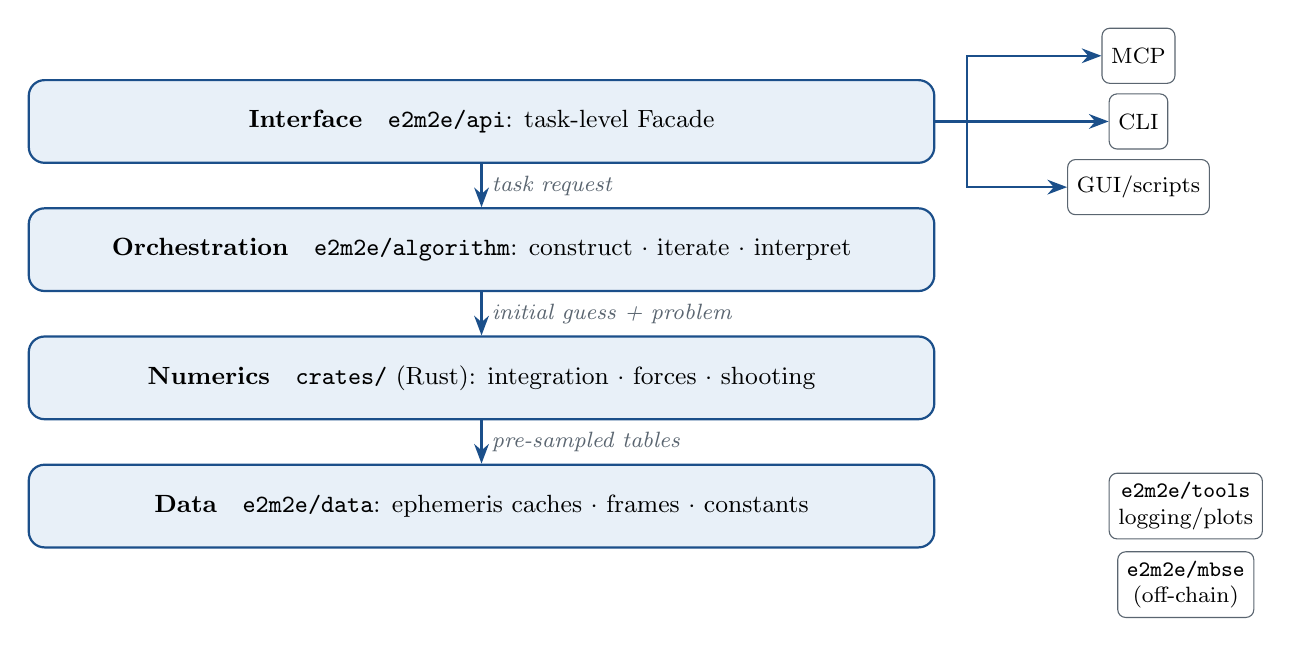
\begin{tikzpicture}[
  font=\small,
  layer/.style={draw=e2blue, thick, rounded corners=2mm, fill=e2light,
    minimum width=11.5cm, minimum height=1.05cm, align=center},
  sub/.style={draw=e2gray, rounded corners=1mm, fill=white,
    minimum height=0.7cm, align=center, font=\footnotesize},
  arr/.style={-{Stealth[length=2.5mm]}, thick, e2blue},
  lbl/.style={font=\footnotesize\itshape, text=e2gray},
]
\node[layer] (api) at (0,0) {\textbf{Interface}\quad \texttt{e2m2e/api}: task-level Facade};
\node[sub, right=2.2cm of api.east, anchor=west] (cli) {CLI};
\node[sub, above=0.12cm of cli] (mcp) {MCP};
\node[sub, below=0.12cm of cli] (gui) {GUI/scripts};
\draw[arr] (api.east) -- (cli.west);
\draw[arr] (api.east) ++(0.4,0) |- (mcp.west);
\draw[arr] (api.east) ++(0.4,0) |- (gui.west);

\node[layer, below=0.55cm of api] (algo) {\textbf{Orchestration}\quad \texttt{e2m2e/algorithm}: construct $\cdot$ iterate $\cdot$ interpret};
\node[layer, below=0.55cm of algo] (rust) {\textbf{Numerics}\quad \texttt{crates/} (Rust): integration $\cdot$ forces $\cdot$ shooting};
\node[layer, below=0.55cm of rust] (data) {\textbf{Data}\quad \texttt{e2m2e/data}: ephemeris caches $\cdot$ frames $\cdot$ constants};

\draw[arr] (api.south) -- (algo.north) node[midway, right, lbl] {task request};
\draw[arr] (algo.south) -- (rust.north) node[midway, right, lbl] {initial guess + problem};
\draw[arr] (rust.south) -- (data.north) node[midway, right, lbl] {pre-sampled tables};

\node[sub, right=2.2cm of data.east, anchor=west] (tools) {\texttt{e2m2e/tools}\\logging/plots};
\node[sub, below=0.15cm of tools] (mbse) {\texttt{e2m2e/mbse}\\(off-chain)};
\end{tikzpicture}
\caption{Runtime layers of e2m2e. Dependencies point downward only: the CLI
and MCP derive from the same Facade source; the orchestration layer constructs
problems but never iterates; the Rust numerical layer holds no SPICE handles
and receives ephemerides as pre-sampled cache tables.}
\label{fig:layers}
\end{figure}

The journey of one orbit task: \texttt{api} receives the request $\to$
\texttt{algorithm/family} picks a family and initial guess $\to$ shooting
sinks into the \texttt{crates} integrators, with per-step forces evaluated by
the forces crate (ephemerides from the pre-sampled cache tables of
\texttt{data/frames}, constants from \texttt{data/constants}) $\to$ the
result lands in the \texttt{catalog/} orbit catalog and is delivered through
the CLI/MCP.

\subsection{Five Architectural Modules}

Above the runtime layers, the engineering organization is divided into five
architectural modules (Table~\ref{tab:modules}). The two are different
viewpoints: the layers describe how computation flows; the modules describe
how the project is maintained.

\begin{table}[htbp]
\centering\small
\caption{The five architectural modules}
\label{tab:modules}
\begin{tabularx}{\textwidth}{@{}lX@{}}
\toprule
\textbf{Module} & \textbf{Responsibilities} \\
\midrule
Spacetime \& constants & Time scales (UTC/TDB/TAI/TT; dynamics standardized on
TDB); frame conversion (J2000/ITRF93/IAU\,2006, GCRS--EBCRS, dynamic axes);
physical constant baselines (DE421/DE440/WGS84 coexisting, single-sourced
across Python/Rust against drift) \\
Rust computation & Six crates (above); iterative problems are constructed by
Python and passed in, Rust only iterates to convergence; ephemerides injected
as cache tables, enabling parallelism \\
Python orchestration & Construct problems, call Rust iterators, interpret
results; three tiers: task-level Facade, design chains (family initial guess
$\to$ Rust correction $\to$ high-fidelity propagation), subproblem
construction \\
CI & Three-platform wheel matrix (Windows x64, Linux x86\_64, Linux aarch64)
+ sdist + GitHub Release + PyPI; CSPICE build packages ship via GitHub
Release; the manylinux 2\_28 glibc baseline covers domestic distributions \\
Data management & GitHub Release manages build libraries and ephemeris data;
Git tracks orbit-family seed parameters; local artifacts enter the orbit
catalog (JSON metadata + NPZ array segments, SQLite only as a derived index) \\
\bottomrule
\end{tabularx}
\end{table}

\begin{keybox}{Design Note}
The boundary of numerical sinking is decided by iteration density: shooting,
continuation, NSGA-II evolutionary operators, and low-thrust direct-method
kernels already live on the Rust side; Python keeps outer orchestration and
reference paths. The constraint that the Rust layer holds no SPICE handles
makes the whole numerical kernel inherently thread-safe and parallelizable
with Rayon. Per-module migration progress is itemized in
\texttt{docs/architecture/numerics-migration-status.md}.
\end{keybox}

\section{Spacetime Reference and Dynamical Kernel}
\label{sec:dynamics}

\subsection{Spacetime Reference: Time, Frames, Constants}

Orbit-computation errors often originate not in algorithms but in reference
baselines. e2m2e maintains the spacetime reference as a dedicated module:

\textbf{Time.} Internally, dynamics standardize on barycentric dynamical time
TDB (SPICE ET seconds or JD\_TDB); UTC appears only at interface boundaries.
The conversion chain covers UTC / TAI / TT / TDB, with leap-second kernels
loaded automatically.

\textbf{Frames.} A coordinate system is decomposed into \textbf{Axes +
Origin}: given an epoch, the axes return a rotation matrix and the origin
returns its absolute state; together they form a complete mathematical
reference frame. Axes types cover the ICRS inertial frame, SPICE
high-precision ITRF93 (verified against \texttt{pxform/sxform} to
$10^{-12}$), a GMAT-compatible ITRF, IAU 2006 simplified Earth orientation
(for SPICE-free scenarios), and the dynamic axes VNB and LVLH that depend on
the spacecraft's instantaneous state (customary for thrust directions and
station keeping). Batch conversion between the synodic frame and J2000 has
sunk to Rust, including the barycenter$\to$geocenter translation correction.

\textbf{Joint spacetime transformation.} Built on the r2s2 library (a
cislunar spacetime coordinate library), the TDT+GCRS $\leftrightarrow$
TDB+EBCRS transformation includes the relativistic terms required by IAU
resolutions; e2m2e fills the EBCRS origin gap ($\vect x_{\mathrm{ebcrs}} =
\vect x_s - \vect x_{\mathrm{emb}}(t)$). Round-trip verification: position
difference $< 0.001$ mm, time difference $< 1\,\mu$s; relativistic
corrections amount to about 0.20 m at LEO altitude and 10.1 m at lunar
distance.

\textbf{Constants.} Physical constants are managed as baselines (DE421 /
DE440 / WGS-84 coexisting, each internally self-consistent, chosen per
scenario), generated single-sourced for both Python and Rust to prevent
drift. The Earth--Moon CR3BP baseline takes the DE421 self-consistent values:
$\mu = 0.01215058535$, characteristic length DU $= 384400$ km, characteristic
time TU $\approx 375190$ s ($\approx 4.34$ days).

\subsection{Three Layers of Dynamical Models}

e2m2e provides three dynamical models at increasing fidelity, with state
conversion among them (Table~\ref{tab:dynamics}).

\begin{table}[htbp]
\centering\small
\caption{Three layers of dynamical models}
\label{tab:dynamics}
\begin{tabularx}{\textwidth}{@{}llX@{}}
\toprule
\textbf{Model} & \textbf{Fidelity} & \textbf{Use and properties} \\
\midrule
CR3BP & Concept design & Dimensionless autonomous system in the synodic
frame, with the Jacobi integral and five libration points; the carrier of
periodic orbit family design \\
BCR4BP & Intermediate & Adds an analytic solar perturbation (Sun position as
an analytic function of time, no ephemeris needed); time-periodic; the
carrier of WSB searches \\
Ephemeris $N$-body & High fidelity & J2000 inertial frame in physical units,
$N$ configurable bodies queried from SPICE ephemerides; accurate mission-level
extrapolation \\
\bottomrule
\end{tabularx}
\end{table}

The circular restricted three-body problem (CR3BP) is a dimensionless
autonomous system in the synodic rotating frame:
\begin{equation}
  \ddot{x} - 2\dot{y} = \frac{\partial\Omega}{\partial x}, \qquad
  \ddot{y} + 2\dot{x} = \frac{\partial\Omega}{\partial y}, \qquad
  \ddot{z} = \frac{\partial\Omega}{\partial z},
\end{equation}
with pseudo-potential and gravitational distances
\begin{equation}
  \Omega = \frac{1}{2}(x^2 + y^2) + \frac{1-\mu}{r_1} + \frac{\mu}{r_2}, \qquad
  r_1 = \sqrt{(x+\mu)^2 + y^2 + z^2}, \quad
  r_2 = \sqrt{(x-1+\mu)^2 + y^2 + z^2},
\end{equation}
and the only integral of motion, the Jacobi constant $C_J = 2\Omega - v^2$.

The bicircular restricted four-body problem (BCR4BP) superposes a solar
point-mass perturbation (direct + indirect terms) on the CR3BP, with the Sun
position given analytically, $\vect r_s(t) = a_s(\cos\theta, \sin\theta, 0)$,
$\theta = \theta_0 + \omega_s t$, retrograde in the synodic frame. The system
is no longer autonomous but remains time-periodic, and serves as the working
medium for WSB ballistic-capture searches: against the ephemeris model, the
1-day extrapolation deviation is about $10^3$ km, and it outperforms the
CR3BP within 2 days.

The ephemeris $N$-body model takes a central point mass plus third-body
perturbations:
\begin{equation}
  \vect a = -\frac{\mu_0\,\vect r}{\norm{\vect r}^3}
  - \sum_i \mu_i \left[
    \frac{\vect r - \vect r_i}{\norm{\vect r - \vect r_i}^3}
    + \frac{\vect r_i}{\norm{\vect r_i}^3}
  \right],
\end{equation}
with body states from SPICE ephemerides---non-autonomous, without libration
points or a Jacobi integral---for mission-level precise design. All three
layers support 42-dimensional augmented STM propagation
($\delta\vect x(t) = \stm(t, t_0)\,\delta\vect x(t_0)$).

\subsection{High-Fidelity Force Models}

On top of the ephemeris layer, force models are managed as a composable
container with registration and per-entry enable/disable; each component
provides an analytic Jacobian and a Rust serialization hook:

\begin{itemize}
  \item \textbf{Gravity}: central point mass; third-body direct + indirect
        terms; fully normalized spherical-harmonics gravity field (Pines
        recursion, supporting EGM96 / GRGM900C and custom coefficient files,
        with built-in Earth solid tides and a lunar $k_2 = 0.024116$ solid
        tide);
  \item \textbf{Solar radiation pressure}: cannonball model
        ($P_{1\mathrm{AU}} = 4.56\times10^{-6}$ N/m$^2$, optional conical
        shadow model with multi-occulter composition aligned with GMAT) and
        the ECOM 9-parameter empirical model (DFH-compatible);
  \item \textbf{Atmospheric drag}: computed in ITRF with default
        $C_d = 2.2$; density from the USSA76 piecewise-exponential atmosphere
        with first-order F10.7 / Ap corrections;
  \item \textbf{Thrust}: continuous thrust (direction frame selectable among
        inertial / VNB / LVLH) and variable-mass continuous thrust (mass as a
        7th state component, 7-dimensional augmented Rust path); impulsive
        maneuvers applied piecewise;
  \item \textbf{Relativistic correction}: post-Newtonian Schwarzschild +
        Lense--Thirring + de Sitter terms, aligned with GMAT.
\end{itemize}

Accuracy: full force-model propagation aligns with GMAT and DFH to the
sub-100\,m level; against a full DFH configuration, a 7-day Halo arc deviates
by 88 m and a 7-day Lissajous arc by 201 m, with 97\% of the residual due to
the intrinsic difference between the ECOM and cannonball SRP models. Per
ADR 0013, GMAT/DFH serve only as development-time cross-references;
correctness is arbitrated by physical definition.

\subsection{The Rust Integrator Kernel}

All heavy iteration runs on the Rust side, which provides three integrator
families (Table~\ref{tab:integrators}). Adaptive RK error control uses the
threshold $\mathrm{tol}\cdot\max(1, \norm{y})$; augmented STM components do
not participate in step-size control (consistent with GMAT). Benchmark
(normalized LEO+J2, 1 day, tol $=10^{-13}$): PD45 takes about 5000 steps
$\times$ 7 evaluations, RK89 about 800 steps $\times$ 16 evaluations, and ABM
about 500 steps $\times$ 2 evaluations---higher-order and multistep methods
significantly reduce the total number of right-hand-side evaluations.

\begin{table}[htbp]
\centering\small
\caption{The three Rust integrator families}
\label{tab:integrators}
\begin{tabularx}{\textwidth}{@{}lllX@{}}
\toprule
\textbf{Family} & \textbf{Methods} & \textbf{Order} & \textbf{Typical use} \\
\midrule
Adaptive single-step RK & PD45 / PD78 / RK89 & 5 / 8 / 9 & General
propagation and accuracy baselines \\
Adams multistep & ABM (PECE) & 4 & Long arcs with smooth dynamics; only 2
RHS evaluations per step \\
Cowell double integration & Störmer--Cowell & 8 & Pure-gravity orbits; state
dimension halved \\
\bottomrule
\end{tabularx}
\end{table}

Two performance-critical designs: first, the \textbf{ephemeris cache}---SPICE
queries are pre-sampled on a uniform grid and injected into Rust as cubic
splines ($C^2$ continuous), accelerating full force-model propagation by more
than $10\times$ while removing the CSPICE global-state constraint on
parallelism; second, the \textbf{compiled path}---once the force model is
serialized, the entire integration loop runs inside Rust with no Python
round-trips. Event detection follows scipy semantics (\texttt{terminal} /
\texttt{direction}), and Poincar\'e sections can directly generate event
functions for in-integration detection.

\section{Periodic Orbit Design}
\label{sec:orbit}

\subsection{An Overview of Orbit Families}

Usable cislunar orbits fall into four layers by distance from the Moon, with
scale as the main thread: the farther from the Moon, the larger Earth's share
of the gravity field, the dynamics transition from two-body Keplerian to
three-body, and orbits turn from stable to unstable
(Table~\ref{tab:families}). e2m2e provides a unified family-generation entry,
\texttt{orbit\_family\_generation()}, covering eight orbit families; Lyapunov
and resonant orbits (RO) are additionally supported at the differential
correction strategy layer.

\begin{table}[htbp]
\centering\small
\caption{Periodic orbit families}
\label{tab:families}
\begin{tabularx}{\textwidth}{@{}llX@{}}
\toprule
\textbf{Family} & \textbf{Location} & \textbf{Characteristics and uses} \\
\midrule
DRO & Moon-centered & Distant retrograde orbit; neutrally stable with low
maintenance cost; candidate for lunar orbital stations \\
DPO & near L2 & Distant prograde orbit; unstable; usable for far-side
communication relay \\
Halo / NRHO & L1/L2 & Three-dimensional periodic orbits; NRHOs are the
high-amplitude near-rectilinear form ($A_z > 0.1$ dimensionless), adopted by
Gateway \\
Axial & L1/L2 & G\'omez Type B bifurcation; axial motion, coverage
complementary to Halo \\
Lyapunov & L1/L2/L3 & Planar periodic orbits \\
Lissajous & L1/L2/L3 & Quasi-periodic (incommensurate in-plane/out-of-plane
frequencies), generated on the nonlinear center-reduced flow \\
SPO / LPO & L4/L5 & Short-/long-period orbits; large-amplitude LPOs take a
horseshoe shape \\
Horseshoe & L4/L5 & Large-amplitude members of the LPO chain \\
RO & --- & Resonant orbits, departing from the $y$-axis symmetry \\
\bottomrule
\end{tabularx}
\end{table}

Periodicity semantics are strictly distinguished: Halo, NRHO, Axial, SPO,
LPO, Horseshoe, and DRO members are strictly periodic; Lissajous members are
quasi-periodic bounded trajectories and are not forced into periodic closure.

\subsection{Initial Guesses: Starting from Analytic Approximations}

The first building block of periodic orbit design is the initial guess, for
which e2m2e has three sources:

\begin{itemize}
  \item \textbf{Richardson third-order analytic approximation} (1980): a
        third-order analytic solution for Halo orbits near the collinear
        libration points. The internal pipeline: solve the libration-point
        distance parameter $\gamma$ (quintic equation, Brent's method) $\to$
        compute the in-plane frequency $\omega_p$ $\to$ assemble the
        third-order coefficients and solution. Small-amplitude seeds (e.g.
        dimensionless $z_0 = 0.001$) are the most accurate and are then
        amplified by continuation;
  \item \textbf{Seed orbits}: the DRO family starts from a standard seed
        (amplitude $\approx 90786$ km), differentially corrected with the
        $x$-axis crossing fixed and continued bidirectionally, covering an
        envelope of 1737--110000 km;
  \item \textbf{Normal-form characteristic parameters}: the dynamics near a
        libration point are reduced to action--angle characteristic
        parameters $[q_1, p_1, I_2, \theta_2, I_3, \theta_3]$, describing
        with a few constants an orbit that would otherwise need six state
        components evolving in time. The pipeline: ephemeris initial state
        $\to$ dynamical substitute orbit $\to$ quasi-Floquet transformation
        $\to$ center-manifold reduction $\to$ characteristic parameters. The
        quasi-Floquet reduction offers a 36-dimensional matrix method or a
        21-dimensional $\mathfrak{sp}(6)$ Lie-algebra parameterization
        (symplectic by construction); the center-manifold Lie transformation
        is truncated at order 10 by default.
\end{itemize}

\subsection{Differential Correction: STM Newton Iteration via Symmetries}

Differential correction iteratively adjusts the initial conditions so that
the orbit satisfies periodicity constraints, at its core an STM-based Newton
iteration. e2m2e exploits the three mirror symmetries of the CR3BP to shrink
the problem---for example, XZ-plane symmetry means that if
$(x, y, z, \dot x, \dot y, \dot z)$ is a solution, so is
$(x, -y, z, -\dot x, \dot y, -\dot z)$; a Halo orbit therefore only needs to
depart perpendicularly from the XZ plane ($y = 0$) and be corrected to cross
it perpendicularly again half a period later.

Different combinations of symmetry and fixed parameters form 11 correction
strategies (Lyapunov/DRO with fixed $x_0$, fixed-period orbits with fixed
$T_{1/2}$, RO with fixed $y_0$, Halo with fixed $z_0$ or $x_0$, Axial with
fixed $v_{z0}$, SPO/LPO at L4/L5 without symmetry and full-period closure,
etc.). Architecturally, the strategy layer is strictly separated from the
solver: strategy functions only produce immutable configuration objects, and
execution sinks to the Rust CR3BP correction kernel.

Convergence failures are diagnosable: the history records per-step errors and
the termination cause (converged / correction below machine precision /
diverged / singular Jacobian / stagnated / converged to a parasitic root with
$T \approx 0$); a singular Jacobian indicates linearly dependent constraints
and calls for a different strategy.

\subsection{Multiple Shooting: Ephemeris Correction of Long Arcs}

Differential correction is sensitive to the initial guess, increasingly so
for longer arcs. Multiple shooting splits the orbit into $N$ independently
integrated segments and imposes continuity constraints at the patch points:
\begin{equation}
  \vect{x}_i(t_{i+1}) = \vect{x}_{i+1}(t_{i+1}),
\end{equation}
adjusting all segment initial states (optionally including time nodes)
simultaneously---turning ``long-arc sensitivity'' into ``many small
corrections''. The standard implementation reaches a tolerance of $10^{-10}$.

Patch-point correction under the ephemeris model uniformly goes through the
Rust multiple-shooting kernel, dispatched by orbit stability along two paths:

\begin{itemize}
  \item \textbf{Stable orbits} (DRO): a velocity-weighted two-level
        path---after correcting one revolution, free extrapolation remains
        bounded;
  \item \textbf{Unstable orbits} (Halo/NRHO/DPO): segmented full-arc
        shooting, integrating segment by segment to fill the ephemeris grid;
        NRHO fixes 1 revolution per segment, Halo at most 3, and DPO uses 64
        equally-spaced patch points per revolution.
\end{itemize}

Node sampling is likewise tailored to orbital physics: Halo uses
perilune-clustered sampling (5 nodes inside the perilune window plus 8
outside), because the STM is ill-conditioned where the velocity is large
near perilune; NRHO uses equal-time sampling.

\subsection{Continuation: From One Orbit to a Family}

Given a converged seed orbit, a family is generated by stepping along a
family parameter (Jacobi constant, amplitude, etc.), reconverging with
differential correction at each step. Two continuation schemes are provided:

\begin{itemize}
  \item \textbf{Natural-parameter continuation}: advances along a single
        parameter, each step seeded by the current solution;
  \item \textbf{Pseudo-arclength continuation (PAL)}: adds an arclength
        constraint and can pass turning points, suitable for families with
        non-monotonic parameter--amplitude relations (e.g. the Halo
        amplitude--period curve).
\end{itemize}

Failure handling is engineered: a non-converged step retries with a reduced
step size; if convergence still fails at the lower bound, that direction
terminates; only converged members are appended to the family, with
diagnostics reporting total/successful/failed steps. The L2 NRHO family uses
a dedicated ``fold then continue with fixed $x_0$'' arrangement; the Halo
family uses natural continuation with fixed $z_0$, positive and negative
$z_0$ giving the northern and southern families.

\subsection{Stability Analysis and Invariant Manifolds}

The stability of a periodic orbit is determined by its monodromy matrix (the
STM over one period):
\begin{equation}
  \mat{M} = \stm(T, 0).
\end{equation}
By the symplectic structure of Hamiltonian systems, eigenvalues appear in
reciprocal pairs $(\lambda, 1/\lambda)$. The Broucke stability index sums
each reciprocal pair:
\begin{equation}
  \nu = \lambda + \frac{1}{\lambda},
\end{equation}
with $|\nu| < 2$ stable and $|\nu| > 2$ unstable (the larger, the more
unstable). The relation of eigenvalues to $+1$, $-1$, and the unit circle
identifies bifurcation types (saddle-node / period-doubling / torus), with
family-level bifurcation detection supported. Numerical trustworthiness is
self-checked via symplectic residuals: if $|\det \mat{M} - 1|$ or
$\norm{\mat{M}^\top \mat{J} \mat{M} - \mat{J}}$ is significantly large, the
integration tolerance should be tightened and the analysis redone.

The real eigenvectors of the monodromy matrix also give the invariant
manifold directions: the stable manifold takes the $|\lambda| < 1$ direction
and the unstable manifold the $|\lambda| > 1$ direction. Transporting the
eigenvectors along the orbit by the STM and applying a $\pm\varepsilon$
perturbation (typically 50 km/DU) yields manifold seeds; integrating
backward/forward produces the manifold tubes used for low-energy transfer
stitching (Section~\ref{sec:transfer}).

\subsection{The Design Pipeline}

Chaining these algorithms together, the complete pipeline of one mission
orbit is:

\begin{center}
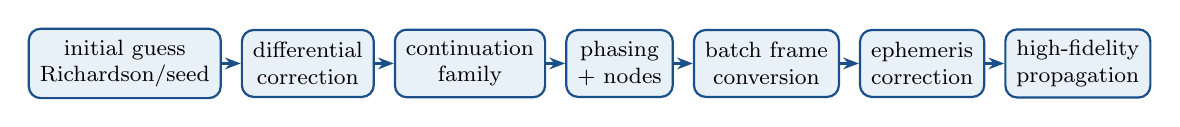
\begin{tikzpicture}[
  font=\footnotesize,
  stage/.style={draw=e2blue, thick, rounded corners=1.5mm, fill=e2light,
    minimum height=0.85cm, align=center, inner sep=4pt},
  arr/.style={-{Stealth[length=2mm]}, thick, e2blue},
]
\node[stage] (s1) {initial guess\\Richardson/seed};
\node[stage, right=0.24cm of s1] (s2) {differential\\correction};
\node[stage, right=0.24cm of s2] (s3) {continuation\\family};
\node[stage, right=0.24cm of s3] (s4) {phasing\\+ nodes};
\node[stage, right=0.24cm of s4] (s5) {batch frame\\conversion};
\node[stage, right=0.24cm of s5] (s6) {ephemeris\\correction};
\node[stage, right=0.24cm of s6] (s7) {high-fidelity\\propagation};
\draw[arr] (s1) -- (s2);
\draw[arr] (s2) -- (s3);
\draw[arr] (s3) -- (s4);
\draw[arr] (s4) -- (s5);
\draw[arr] (s5) -- (s6);
\draw[arr] (s6) -- (s7);
\end{tikzpicture}
\end{center}

All numerical heavy lifting (propagation, shooting, batch frame conversion,
batch ephemeris queries) runs on the Rust side, with Python only
orchestrating; the end-to-end generation of four typical orbits (LLO, ELFO,
DRO, Halo) takes under one minute in total with a release build.

\begin{keybox}{NominalOrbit: The Contract Between Design and Control}
A designed nominal orbit is delivered as a NominalOrbit structure: an
equally-spaced state table + a Floquet basis + projection factors.
Station-keeping algorithms consume this structure directly---the Floquet
analysis produced during design does not need to be recomputed during
control; the two stages are decoupled through a single data contract.
\end{keybox}

\section{Transfer Orbit Design}
\label{sec:transfer}

Transfer design in e2m2e covers impulsive, low-energy, and low-thrust
propulsion modes. The core methodology is a two-step ``search then optimize''
scheme: ballistic propagation on a coarse grid first filters the feasible
solution families, then the best candidates are handed to nonlinear
programming (NLP) for refinement. The unified design variables are the
tangential velocity ratio $\alpha$ (controlling the departure direction), the
transfer time $T$, and the time $t_{\mathrm{ins}}$ from apoapsis to the
insertion point, with the total objective
\begin{equation}
  J = \Delta v_1 + \Delta v_2 ,
\end{equation}
subject to position continuity at the insertion point, velocity-direction
parallelism with the target, and collision avoidance with the Earth and the
Moon. The dynamical baseline is the CR3BP, with $\mu$ taken from the DE421
constant baseline.

\subsection{Impulsive Transfers}

\subsubsection{Lambert Solving and Porkchop Scans}

The Lambert solver implements the Izzo (2015) algorithm with a Rust kernel
(Python only converts and wraps): it supports short-/long-way directions and
multi-revolution solutions (returning the low-energy right branch), and
provides a batch interface---a grid of $N$ geometries $\times\,M$ times of
flight enters Rust in one call, with infeasible combinations filled with NaN
without affecting the rest. The solver is verified against Vallado's classic
test case.

Solving Lambert point by point over a departure-epoch $\times$ time-of-flight
grid yields the porkchop two-impulse $\Delta V$ map; terminal states are
extracted through the terminal-condition abstraction
(\texttt{TerminalCondition}), and analytic terminals need no dynamics
propagation.

\subsubsection{Three-Body Targeting}

A two-body Lambert solution only qualifies as an initial guess in cislunar
space. The three-body Lambert targeter seeds a damped Newton iteration in the
CR3BP with the two-body solution: propagating with the state transition
matrix $\stm(t, t_0)$, each correction is solved from the $\stm_{rv}$ block
of the terminal STM; the step is halved whenever a full step increases the
error; convergence is declared when the terminal position error falls below
$10^{-8}$ (dimensionless).

\subsubsection{Multi-Impulse Optimization and the Lawden Primer-Vector Test}

For an $n$-impulse transfer between fixed endpoints, the decision variables
are only the intermediate nodes $[t_i, \vect{r}_i]$; arcs between adjacent
nodes are closed by Lambert solutions (optionally refined by three-body
targeting), and SLSQP minimizes the total $\Delta V$. Whether a two-impulse
solution can still be improved is answered by the Lawden primer-vector test:
from the transversality conditions $\vect{p}(t_0) = \hat{\Delta v}_0$ and
$\vect{p}(t_f) = \hat{\Delta v}_f$, the costate is carried by the STM to give
the $\vect{p}(t)$ curve, with the necessary optimality condition
\begin{equation}
  \norm{\vect{p}(t)} \le 1 \quad \text{throughout},
  \qquad \norm{\vect{p}} = 1 \text{ at impulses, aligned with them}.
\end{equation}
If $\norm{\vect{p}} > 1$ within an arc, inserting an intermediate impulse
reduces the total $\Delta V$ (Lion \& Handelsman, 1968); the test also
reports the suggested insertion time and position, directly seeding a
three-impulse optimization. A LEO$\to$GEO example reproduces the Hohmann
benchmark of $3.7708$ km/s.

The classical Hohmann two-impulse minimum-energy transfer
\begin{equation}
  \Delta v_1 = \sqrt{\frac{\mu}{r_1}}\left(\sqrt{\frac{2 r_2}{r_1+r_2}} - 1\right),
  \qquad
  \Delta v_2 = \sqrt{\frac{\mu}{r_2}}\left(1 - \sqrt{\frac{2 r_1}{r_1+r_2}}\right)
\end{equation}
is provided as an analytic benchmark and a source of initial guesses.

\subsection{Low-Energy Transfers}

\subsubsection{Lunar Gravity Assist (LGA)}

A three-leg conic-patching design: hyperbolic departure from the initial
orbit $\to$ a gravity assist inside the lunar sphere of influence that
rotates the velocity vector $\to$ hyperbolic insertion into the target orbit.
The search interface works in dimensionless CR3BP states; a typical search
domain is 15--45 days of flight time with a total $\Delta v$ cap of
4.0 km/s, and results report total cost, flight time, and perilune altitude.

\subsubsection{WSB Ballistic Capture}

The weak stability boundary (WSB) route exploits the Sun--Earth weakly stable
region: the spacecraft leaves the lunar sphere of influence onto a distant
Sun-perturbed arc, where solar gravity does work near apoapsis so that the
Moon-relative velocity drops below the capture threshold, yielding ballistic
capture at near-zero $\Delta v$ (Belbruno \& Miller, 1993). The capture
criterion is a negative two-body Kepler energy at perilune:
\begin{equation}
  H_2 = \frac{\norm{\vect{v}}^2}{2} - \frac{\mu_{\mathrm{moon}}}{r} < 0 .
\end{equation}
The solution proceeds in two steps: a \textbf{ballistic grid search}
propagates forward in the BCR4BP over a Sun-phase $\times$ departure-phase
$\times$ flight-time grid, filtering by perilune altitude and the $H_2$
criterion---propagation, section detection, and filtering all run in Rust
with Rayon parallelism (the Python reference implementation runs only when
explicitly requested, never as an automatic fallback); an \textbf{arrival-leg
refinement} then closes the best candidate's Moon-centered arrival arc with
three-body Lambert targeting. A typical search domain is 90--150 days.

\subsubsection{Invariant-Manifold Stitching}

A third low-energy route exploits the invariant manifold tubes of periodic
orbits themselves: crossings of the departure orbit's unstable manifold and
the target orbit's stable manifold on the same Poincar\'e section (a planar
section, or a periapsis section $s = \vect r \cdot \vect v = 0$) are paired
and ranked by the weighted patching cost
\begin{equation}
  w_r \norm{\Delta \vect r} + w_v \norm{\Delta \vect v}.
\end{equation}
The end-to-end pipeline: propagate the departure unstable manifold $\times$
target stable manifold (all four $\pm$ branch combinations, globally best
taken) to the secondary's periapsis section, pick the best patch, then close
onto the target orbit after the patch point with three-body Lambert
targeting; impulses accordingly split into departure, patch, and arrival
segments. In the benchmark case (medium-to-large-amplitude members of the L1
Lyapunov family), the patch impulse is on the order of tens of m/s. The route
is currently CR3BP-based, with an ephemeris interface reserved.

The value of low-energy routes: trading time for propellant, enabling
economical lander/orbiter scenarios and even emergency low-fuel rescue
corridors.

\subsection{Low-Thrust Transfers}

The low-thrust leg uses the 7-dimensional augmented state
$[\vect{r}, \vect{v}, m]$:
\begin{equation}
  \dot{\vect r} = \vect v, \qquad
  \dot{\vect v} = \vect a_{\mathrm{grav}} + \frac{T\,\delta}{m}\,\hat{\vect u}, \qquad
  \dot m = -\frac{T\,\delta}{I_{sp}\, g_0},
\end{equation}
with throttle $\delta \in [0,1]$ and thrust direction $\hat{\vect u}$
parameterized by spherical angles $(\theta_1, \theta_2)$. Solving is a
two-level loop: a \textbf{Q-law initial guess} integrates a Lyapunov feedback
law forward to produce a suboptimal control history; an \textbf{SLSQP
polish} then minimizes propellant over piecewise-constant controls
$(\delta, \theta_1, \theta_2)$ per segment, matching the terminal position
and velocity. Two solvers are available: shooting (analytic Jacobians,
5--24$\times$ faster) and Hermite--Simpson collocation (more robust at large
scale).

Impulsive and low-thrust costs are distinguished via the equivalent
$\Delta v$: impulsive uses $\Delta v = \sum_i \norm{\Delta \vect v_i}$, while
low-thrust inverts the Tsiolkovsky equation,
$\Delta v_{\mathrm{eq}} = I_{sp}\, g_0 \ln(m_0/m_f)$; due to gravity losses,
$\Delta v_{\mathrm{eq}} \ge$ the impulsive $\Delta V$, with significant
differences on high-energy transfers.

\subsection{The Grid-Search + NLP Two-Step Optimization Framework}

Step one, \textbf{grid search}: departure points are sampled equally in time
along the departure orbit (typically 200), each with $\alpha$ uniformly
sampled in $[0.5, 2.5]$ (typically 101); transfer arcs are integrated forward
and filtered by collision (200 km at Earth / 100 km at the Moon),
intersection, and minimum-distance ($10^{-3}$) constraints; the numerical
kernel has sunk to Rust and runs in parallel.

Step two, \textbf{NLP refinement}: decision variables
$\vect{y} = \{\alpha, T, t_{\mathrm{ins}}\}$, objective
$J(\vect y) = \Delta v_1 + \Delta v_2$, constraints of insertion-point
position continuity (equality) and velocity parallelism (equality, or relaxed
to an inequality with an angular tolerance of 0.05 rad). The solver defaults
to SciPy SLSQP, with the COPT commercial optimizer as an option and fallback
on failure.

\begin{table}[htbp]
\centering\small
\caption{Transfer design capabilities at a glance}
\label{tab:transfer}
\begin{tabularx}{\textwidth}{@{}llX@{}}
\toprule
\textbf{Category} & \textbf{Method} & \textbf{Notes} \\
\midrule
Impulsive & Lambert (Izzo) & Rust kernel, batch grid solving, short/long
way and multi-revolution \\
Impulsive & Three-body targeting & Damped Newton + STM, position error
$< 10^{-8}$ at convergence \\
Impulsive & Multi-impulse & SLSQP + Lawden primer-vector test, automatic
impulse-insertion suggestions \\
Impulsive & Hohmann & Analytic benchmark and initial guesses \\
Low-energy & LGA & Three-leg conic patching, TOF 15--45 days \\
Low-energy & WSB & BCR4BP + $H_2<0$ criterion, Rust Rayon parallel search \\
Low-energy & Manifold stitching & Poincar\'e section pairing + three-body
closure, patch impulses at m/s scale \\
Low-thrust & Q-law + NLP & Shooting (analytic Jacobian, 5--24$\times$) or
collocation \\
Framework & Search--optimize & Grid search (Rust parallel) $\to$ SLSQP/COPT
refinement \\
\bottomrule
\end{tabularx}
\end{table}

\section{Orbit Control and Monte Carlo Simulation}
\label{sec:control}

Unstable orbits (Halo/NRHO/DPO) are only truly usable together with station
keeping. e2m2e makes control simulation the last link of the design chain:
the NominalOrbit produced during design (an equally-spaced state table +
Floquet basis + projection factors) is consumed directly by the control
algorithms, with no need to recompute the Floquet analysis.

\subsection{Three Control Laws}

\begin{itemize}
  \item \textbf{Feature-point control}: corrections are applied only at
        characteristic locations (e.g. perilune or plane crossings)---few
        maneuvers, low propellant cost, suitable for long-term keeping;
  \item \textbf{Strict target-point control}: the state is driven exactly
        back to a target point on the nominal orbit---highest tracking
        accuracy;
  \item \textbf{Relaxed target-point control}: the target point admits an
        error band, trading tracking accuracy against propellant consumption.
\end{itemize}

Angular-momentum management is also provided: joint attitude/thruster control
that folds momentum unloading into the station-keeping strategy.

\subsection{Monte Carlo Error Simulation}

Station-keeping propellant statistics must be evaluated under error models.
e2m2e supports Monte Carlo simulation with jointly injected navigation and
thrust errors: batches of keeping simulations on the same nominal orbit yield
$\Delta V$ consumption distributions and orbit-maintenance statistics, giving
mission studies confidence intervals rather than point estimates. Simulation
artifacts are automatically archived in the orbit catalog with tag
management---in the MCP scenario, ``run 100 Monte Carlo station-keeping
simulations on this NRHO and tag the results \texttt{candidate}'' is a
workflow completed by a single natural-language instruction.

\section{Interfaces, Data, and Ecosystem}
\label{sec:interfaces}

\subsection{The Facade: A Single Task-Level Entry}

All capabilities converge on a single \texttt{Facade} class (ADR 0014), from
which the CLI and the MCP server are derived from the same metadata source:
beyond input validation, the task-level API model also exposes parameter
metadata for the current task context (conditional value domains and
validators share one rule definition), so that GUIs, the CLI, and MCP can
generate widgets and range hints---external consumers keep no local copies of
parameter rules. Task-level methods come in three tiers:

\begin{itemize}
  \item \textbf{Primary tasks}: \texttt{design\_orbit} (mission orbit design:
        CR3BP initial guess $\to$ ephemeris correction $\to$ high-fidelity
        propagation), \texttt{control\_orbit} (station-keeping Monte Carlo
        simulation), \texttt{transfer\_design} (HMN/LGA/WSB/low-thrust),
        \texttt{orbit\_propagation} (orbit propagation), and
        \texttt{spacetime\_transform} (synodic$\leftrightarrow$J2000 and
        GCRS$\leftrightarrow$EBCRS conversions);
  \item \textbf{Secondary subtasks}: \texttt{orbit\_family\_generation}
        (continuation generation of eight families, with family records
        automatically archived), among others;
  \item \textbf{Orbit catalog}: 7 catalog methods (below).
\end{itemize}

\begin{lstlisting}[caption={Designing an Earth--Moon L2 Halo orbit (examples/main\_design.py)},label=lst:quickstart]
from e2m2e.api import Facade

facade = Facade()

result = facade.design_orbit(
    orbit_type="Halo",
    collinear_point=2,
    amplitude=30000.0,          # km
    epoch=[2024, 1, 1, 0, 0, 0.0],
    duration=365.25 * 86400.0,  # s
)

print(result.orbit_type)
print(result.initial_state)
\end{lstlisting}

\subsection{MCP: An Agent-Native Interface}

e2m2e can act as an MCP server (\texttt{e2m2e mcp-serve}, stdio transport,
listening on no port), exposing 13 task-level tools to LLM agents: 6 task
methods (the 5 primary ones plus family generation) and 7 orbit-catalog
tools. The tool list is purely derived from Facade method metadata---nothing
else to maintain. All responses use a unified envelope
\texttt{\{status, data, error, meta\}}: errors are expressed as error codes
(\texttt{INVALID\_PARAMS}, \texttt{RECORD\_NOT\_FOUND},
\texttt{PROPAGATION\_FAILED}, etc.) without leaking tracebacks, and numerical
tools report soft-failure semantics via \texttt{data.status} (converged /
diverged / stagnated / max\_iterations, ADR 0020)---an agent can treat
``not converged'' as normal information rather than an exception.

Setup is a single command registered in the MCP client; it is recommended to
pin \texttt{cwd} to the directory containing \texttt{kernels/} (SPICE
kernels) and \texttt{catalog/} (the orbit catalog), or to give absolute paths
via \texttt{SPICE\_KERNEL\_DIR} / \texttt{E2M2E\_CATALOG\_DIR}. Once
configured, the server can be driven in natural language, e.g.:

\begin{quote}\itshape
Design an L2 southern NRHO with 3000 km perilune altitude, then run 100
Monte Carlo station-keeping simulations on it and tag the results
``candidate''.
\end{quote}

\subsection{The Orbit Catalog}

Computation artifacts are automatically archived (ADR 0031): a record is JSON
metadata + NPZ array segments (with a schema version), with SQLite only as a
derived index. Productive tools return a \texttt{record\_id} on success,
which chains across tools (e.g. \texttt{control\_orbit} can reference the
output of \texttt{design\_orbit} via \texttt{input\_record\_id}). Seven
catalog tools cover the full lifecycle: \texttt{catalog\_query}
(multi-dimensional filtering by family / libration point / Jacobi range /
amplitude / tag / convergence status), \texttt{catalog\_get},
\texttt{catalog\_delete}, \texttt{catalog\_tag} (teaching annotations),
\texttt{catalog\_promote} (promoting a family member to a standalone record),
\texttt{catalog\_export} (packaged export), and \texttt{catalog\_sweep}
(batch generation over parameter grids).

\subsection{Installation and Deployment}

\begin{lstlisting}[style=e2bash,caption={Installation and SPICE kernel setup},label=lst:install]
uv pip install e2m2e            # release wheels embed CSPICE, ready out of the box
uv pip install "e2m2e[mcp]"     # MCP server

# development from source (requires the Rust toolchain):
git clone https://github.com/cislunarspace/e2m2e.git
cd e2m2e
make dev      # sync deps + fetch CSPICE package & SPICE kernels + build the Rust extension
\end{lstlisting}

Release wheels cover Windows x86\_64, Linux x86\_64, and Linux aarch64
(Kunpeng / Phytium / Raspberry Pi), with statically linked CSPICE embedded,
so the Rust fast paths (STM propagation, shooting, third-body gravity, etc.)
work out of the box; when the extension is unavailable, an explicit error is
raised rather than silently degrading. The SPICE kernels are packaged as the
GitHub Release asset \texttt{kernels-v1} (downloaded automatically by
\texttt{make setup}), including DE planetary ephemerides, Earth rotation,
Moon attitude, leap seconds, and planetary constants kernels; the r2s2
spacetime transformation additionally requires an ephemeris containing the
TT$-$TDB time ephemeris. The official source is NASA NAIF.

The \texttt{examples/} directory provides six runnable examples: end-to-end
orbit design, station-keeping Monte Carlo, high-fidelity propagation, a
Lambert transfer, a four-layer comparison of lunar orbits (LLO/ELFO/DRO/Halo,
under one minute in total), and orbit-family generation.

\section{Comparison with Existing Tools}
\label{sec:comparison}

\subsection{Scope and Method}

This chapter positions e2m2e within the existing aerospace software
ecosystem. Ten comparison subjects cover four shapes: general-purpose mission
analysis platforms (GMAT, STK, ATK), open-source astrodynamics libraries
(Orekit, pykep, poliastro), the starting point of the self-built route and
its accuracy yardstick (SciPy), and ecosystem complements (r2s2, Cesium,
ootk). The survey was completed in September 2026 with e2m2e 5.9.2 as the
version anchor: GMAT, Orekit, pykep, poliastro, ootk, and r2s2 were examined
at the code level (repository-wide greps and source reading), while the
closed-source STK and ATK and the pure-rendering Cesium were surveyed through
official documentation and third-party literature. Every number cited below
can be re-verified in the respective repositories or official documentation.

Three principles keep the narrative fair:

\begin{enumerate}
  \item \textbf{No head-to-head, no multiples}: where same-scenario
        benchmark data are lacking (STK, Orekit, ATK), only architectural
        comparisons are made---no performance multiples are claimed;
  \item \textbf{Partitioned performance claims}: speedups against the SciPy
        self-built route can be quantified (the callback overhead is
        structural); differences from GMAT are stated at the parallelism
        architecture level;
  \item \textbf{Accuracy as alignment, not contest}: e2m2e's force-model
        layer uses GMAT's mathematical specification as its porting baseline,
        so the accuracy relationship is ``alignment statement + component
        porting consistency'', not ``who is more accurate''.
\end{enumerate}

\subsection{Ecosystem Landscape}

\begin{table}[htbp]
\centering\footnotesize
\caption{The comparison landscape (version anchors, August 2026)}
\label{tab:landscape}
\begin{tabularx}{\textwidth}{@{}llXX@{}}
\toprule
\textbf{Tool} & \textbf{Vendor / License} &
\textbf{Positioning (language)} & \textbf{Relationship to e2m2e} \\
\midrule
GMAT & NASA / Apache-2.0 & General mission analysis platform, GUI + plugins
(C++, $\sim$850k LoC) & e2m2e's force-model alignment baseline; no CR3BP
kernel \\
STK & Ansys / proprietary & Digital mission engineering platform &
Industry de facto standard; Astrogator has a CR3BP framework but no family
automation \\
ATK & NUDT / closed binary & Domestic STK counterpart, 300+ organizations &
General MCS framework; no declared three-body design tools \\
Orekit & CS GROUP / Apache-2.0 & Flight dynamics infrastructure library
(Java, $\sim$470k LoC) & The most mature infrastructure; three-body limited
to Halo/Lyapunov components \\
pykep & ESA / MPL-2.0 & Interplanetary trajectory optimization research
library (C++23 + pybind) & Three-body limited to integrators and benchmark
problems; not operational \\
poliastro & community / MIT & Teaching-grade astrodynamics (Python + numba) &
\textbf{Archived} (Oct 2023); three-body stuck in contrib drafts \\
SciPy & community / BSD family & General scientific computing (Python +
C/Fortran) & Starting point of the self-built route and e2m2e's accuracy
yardstick \\
ootk & thkruz / AGPL-3.0 & Web Earth-orbit SSA toolkit (TypeScript) &
Different track; near-zero overlap; complementary \\
r2s2 & PMO CAS / GPL-3.0 & Relativistic spacetime coordinate conversion
(Python, $\sim$1.2k LoC) & \textbf{e2m2e's underlying dependency}, not a
competitor \\
Cesium & Cesium GS / Apache-2.0 & 3D visualization engine (JS/TS, WebGL) &
Pure rendering, zero computation; a natural front end \\
\bottomrule
\end{tabularx}
\end{table}

\subsection{The Core Differentiation Axis: Cislunar Three-Body Design
Automation}
\label{subsec:three-body-axis}

The watershed between e2m2e and every comparison subject is whether the
three-body capability is a \emph{design pipeline} or merely \emph{parts and
frameworks} (Table~\ref{tab:threebody}).

\begin{table}[htbp]
\centering\small
\caption{Cislunar three-body capability comparison (the core differentiation
axis)}
\label{tab:threebody}
\begin{tabularx}{\textwidth}{@{}lXX@{}}
\toprule
\textbf{Tool} & \textbf{CR3BP dynamics / family generation} &
\textbf{Low-energy transfer / station keeping / ephemeris correction} \\
\midrule
\textbf{e2m2e} & \textbf{Native} three-model (CR3BP/BCR4BP/ephemeris
$N$-body) conversions; \textbf{automatic generation of eight families} +
continuation + energy-window batch scanning & Manifold stitching + LGA/WSB;
three control laws + Monte Carlo; the initial-guess $\to$ ephemeris
correction (20 m convergence) $\to$ high-fidelity three-stage chain \\
GMAT & No CR3BP module (repository-wide grep: zero hits); libration points
are geometric points only, rotating frames assembled by users & None; the
ephemeris propagator is a replay-style propagator \\
STK & Astrogator has a built-in CR3BP force model + differential targeting
since 11.7 & No templated family generation (no public evidence found);
low-energy transfers assembled in MCS; no keeping control laws \\
ATK & High-precision $N$-body numerical propagation + general MCS (11
segment types $\times$ 60 constraints) & Family generation/manifolds not
claimed in public materials; a paper reproducing GMAT's Halo keeping case \\
Orekit & CR3BPForceModel + STM, component-style & Only Halo/Lyapunov two
types; manifolds as single-point initial values only; no keeping; shooter
accepts ephemeris models (user-assembled) \\
pykep & heyoka symbolic factory + 42-dimensional variational equations & No
family generation (grep: zero hits); no manifolds; 14 cislunar low-thrust
\textbf{benchmark problems}---whose inputs are precisely e2m2e's outputs \\
Others & SciPy: zero orbit knowledge; poliastro: three-body in contrib
drafts; ootk/Cesium: no three-body code & --- \\
\bottomrule
\end{tabularx}
\end{table}

The conclusion is clear: \textbf{none of the eight comparison subjects
combines ``eight-family generation + manifold low-energy transfer +
three-body station keeping + ephemeris correction chain''}. GMAT's three-body
capability is geometric points plus $N$-body summation; STK provides a
framework whose workflows are hand-built sequences; Orekit provides parts
that users must assemble; pykep treats the three-body problem as an
optimization carrier rather than a design object; poliastro's three-body work
never entered the main library. Cislunar three-body design automation is
therefore e2m2e's unique niche.

\subsection{Profiles of Representative Subjects}

\subsubsection{General-Purpose Platforms: GMAT, STK, ATK}

\textbf{GMAT} (NASA, $\sim$850k lines of C++) is the ``closest'' subject to
e2m2e: the PD78/RK89 weights, the conical shadow model, the three
relativistic terms, the STM step-error-control semantics, and the EOP/leap
second fixtures are all ported from the GMAT R2026a mathematical
specification---the force-model layer can be described as ``a Rust
re-implementation and extension of GMAT's mathematical specification''. In
return, GMAT's solver and optimization ecosystem (DifferentialCorrector,
Yukon SQP, the CSALT direct-collocation framework, Bulirsch--Stoer
integrators) and its document-level V\&V system (mathematical specification,
flight-qualification documents) are thickness e2m2e does not yet have; its
lack of a parallel propagation kernel (zero grep hits in physics loops) marks
a generational difference from e2m2e's service-oriented form. The two are in
a ``benchmark and differentiate'' relationship: GMAT for cross-checking and
operations analysis, e2m2e for the three-body design pipeline.

\textbf{STK} (Ansys, proprietary) is the industry's de facto standard.
Astrogator has included the CR3BP force model and differential targeting
since 11.7, and the Artemis II Orion tracking visualization is STK-driven.
The comparison reduces to four axes: license (proprietary commercial vs
Apache-2.0), three-body automation (framework vs one-click family
generation), cost (a government purchase record of USD 114.5k for a single
Pro token vs free), and programmability (an Integration license module vs a
native MCP server). STK's coverage/link/scheduling/ODTK module ecosystem is
outside e2m2e's scope; in typical workflows the two form an ``open-source
computation + commercial presentation'' layering.

\textbf{ATK} (NUDT, closed binary) takes the ``Chinese counterpart of STK''
route: a building-block maneuver planning framework (11 orbit-segment types,
19 stopping conditions, 11 categories / 60 constraint components, unified NLP
with three solver classes---differential correction / SQP / intelligent
optimization), backed by operational support of the Tiangong station, Shenzhou
and Tianzhou missions. Its paper reproduces the lunar free-return case and
GMAT's built-in L2 Halo keeping case (four maneuvers of
$-0.25/1.64/8.05/6.44$ m/s), showing the framework can carry three-body
problems; yet public materials declare no CR3BP propagator, no libration-point
family generation, and no invariant-manifold automation---which remains
e2m2e's cleanest point of difference. ``Platform vs library'', ``closed vs
open'', and ``general MCS vs three-body-dedicated pipeline'' are the three
axes of comparison.

\subsubsection{Open-Source Astrodynamics Libraries: Orekit, pykep, poliastro}

\textbf{Orekit} (CS GROUP, $\sim$470k lines of Java, 24 years of development
since 2002) is the benchmark for engineering-grade infrastructure:
frame/time chains compared element-by-element against the official SOFA
library to $10^{-12}$, a propagator family spanning numerical / analytic /
DSST semi-analytic / SGP4 / GNSS, a full orbit-determination suite (batch
least squares + EKF/UKF), and 80+ event detectors---depth e2m2e does not
have. But its three-body capability is component-style: the dynamics model,
Richardson initial guess, and shooter parts exist, while the orbit-type
enumeration holds only Halo and Lyapunov---no family continuation, no
Lissajous/DRO, no batch manifold propagation and stitching, no keeping
control laws. Both Apache-2.0, ``Orekit for the Earth segment and orbit
determination, e2m2e for cislunar design'' is a natural division of labor.

\textbf{pykep} (ESA, kep3, MPL-2.0) is an interplanetary trajectory
optimization research library: the heyoka LLVM-JIT Taylor integrator
(tolerances to $10^{-16}$) plus pagmo evolutionary optimization, MGA
encodings, Sims--Flanagan/ZOH low-thrust transcriptions, and Pontryagin
indirect methods---officially ``not an operational flight dynamics tool''.
Its three-body capability stops at a symbolic dynamics factory and 14
cislunar low-thrust benchmark problems (TOPS: Halo-to-Halo, DRO-to-NRHO,
etc.); libration-point computation, family construction, monodromy matrices,
and manifold targeting are unimplemented---while the inputs of the TOPS
benchmarks (Halo/DRO/NRHO nominal orbits) are precisely e2m2e's outputs.
``e2m2e generates the nominal orbit $\to$ pykep + pygmo for low-thrust
global optimization $\to$ e2m2e for high-fidelity verification and keeping''
is a ready-made division-of-labor chain.

\textbf{poliastro} (MIT, archived October 2023) matters to this white paper
as \textbf{evidence of an ecosystem vacancy}: its unit-safe API and plotly
visualization are teaching-grade gems, but its cislunar three-body work
remained in the contrib draft directory (its own README lists as unimplemented:
differential correction, family continuation, the third-order Halo analytic
solution, monodromy, manifolds), with only 6 perturbation functions and test
tolerances at the $10^{-4}\sim10^{-2}$ level. The most active
teaching-oriented astrodynamics library in the Python ecosystem is archived
with its three-body agenda unfinished---precisely the vacancy e2m2e fills.

\subsubsection{The Self-Built Route and Accuracy Yardstick: SciPy}

SciPy knows nothing about orbits---no time systems, no reference frames, no
ephemerides, no force models---yet \texttt{solve\_ivp} + \texttt{root}
assembled into a CR3BP targeter is the de facto self-built route in academia,
and the ``lower-bound alternative'' an e2m2e user would try first. On
performance, its explicit RK family is implemented in Python with a
right-hand-side callback at every step, running 1--3 orders of magnitude
slower than compiled kernels on tight-tolerance, batch-targeting workloads
(community consensus; e2m2e's corresponding evidence: the same parallelized
problem yields about $1/10$ of the Rust-sunk speedup under Python
multiprocessing). On accuracy the two are at par---e2m2e's test suite uses
scipy DOP853 ($10^{-13}$) as its gold-standard reference, with a
LEO+J2 one-day-arc consistency of $<10^{-9}$. The gap is not accuracy but
the fact that reaching the same accuracy requires users to build the entire
domain layer themselves.

\subsubsection{Ecosystem Complements: r2s2, Cesium, ootk}

\textbf{r2s2} (Purple Mountain Observatory, CAS; $\sim$1150 lines of pure
Python) is not a competitor but an underlying dependency: the
GCRS$\leftrightarrow$EBCRS relativistic spacetime conversion rides on it,
with reverse conversions converging to 1 ns / 1 mm by default. e2m2e's
independent verification of it (round-trip consistency, differencing against
the SPICE chain, differencing against ERFA \texttt{dtdb}) constitutes its
main test coverage. r2s2 is GPL-3.0; closed-source integrators should note
the copyleft implications.

\textbf{Cesium} (CesiumJS, Apache-2.0) is a pure rendering layer with zero
orbital mechanics---satellite positions must be fed in externally. It was
historically ``built to track objects in space'' and treats cislunar-scale
scenes as first-class citizens (ICRF inertial rendering; the Artemis II
lunar-orbit tracking case). Visualization is exactly e2m2e's weak spot, and
``EphemerisTable $\to$ CZML $\to$ Cesium'' is a license-clean composition
path (Orekit + OreCZML already validate the same template). The division to
remember: Cesium faithfully renders whatever trajectory it is fed; the
correctness of the trajectory is e2m2e's responsibility.

\textbf{ootk} (TypeScript, AGPL-3.0) plays a different sport entirely:
SGP4/TLE cataloging, sensors, conjunctions, Web-side SSA---near-zero overlap
with e2m2e. Its value is twofold: complementarity (catalog/observation
ground to ootk, high-fidelity mission design to e2m2e), and methodology:
ootk regresses against bit-level snapshots of the official AFSPC SGP4Prop
and Vallado's verification vectors, with SLR precise ephemerides as
independent ground truth---the kind of ``bit-level alignment against
authoritative reference implementations'' that e2m2e's verification system
can borrow as it matures.

\subsection{Performance and Accuracy: Partitioned Evidence}

\begin{table}[htbp]
\centering\small
\caption{Parallelism architecture and public quantitative figures}
\label{tab:perf}
\begin{tabularx}{\textwidth}{@{}lXl@{}}
\toprule
\textbf{Tool} & \textbf{Architecture} & \textbf{Public figures} \\
\midrule
\textbf{e2m2e} & Rust kernel + Rayon (shooting/grid/manifolds/WSB) &
Reproducible; benchmark scripts in-repo \\
GMAT & No parallel propagation kernel (single-instance sequential) & none \\
STK & Parallel Computing multi-core distribution & 8 cores, 180 samples,
70 s (only figure found) \\
Orekit & PropagatorsParallelizer & no public figures \\
pykep & heyoka LLVM JIT + per-tolerance caching & SF evaluation
5.25 $\mu$s; ``thousands of trajectories per second'' \\
SciPy & single-threaded, Python RHS callback & 1--3 orders slower than
compiled kernels \\
ootk & pure JS, single-threaded (light compute $\times$ massive calls) &
SGP4 391 ns/call \\
\bottomrule
\end{tabularx}
\end{table}

e2m2e's own performance figures are all reproducible: transfer grid search
accelerated 5.5--10.4$\times$ by sinking to Rust; 180-day Halo end-to-end
design 223 s $\to$ 63 s; shooting 9.4$\times$ faster with SRP on the Rust
STM fast path; low-thrust analytic Jacobians 3--24$\times$. Per the
principles above, these numbers are compared in magnitude only against the
SciPy self-built route and at architecture level against GMAT; no mutual
multiples are claimed against STK/Orekit/ATK---none of them publishes
same-scenario comparison data.

On accuracy (Table~\ref{tab:prec}), anchors and verification philosophies
differ: Orekit's and ootk's element-wise/bit-level comparisons against
authoritative references have the most complete evidence chains; pykep
reaches $10^{-13}$ in dimensionless normalized units; e2m2e achieves
$10^{-9}\sim10^{-11}$ for integrators against analytic solutions,
$<10^{-12}$ for the coordinate chain, and sub-100 m force-model alignment
with DFH (88 m over a 7-day Halo arc)---though, per the
verification-by-definition principle of ADR 0013, the external comparison
tests have been removed from the repository, leaving only self-runnable
GMAT comparison scripts. Accuracy is not the differentiator; the solvable
problem domain is.

\begin{table}[htbp]
\centering\small
\caption{Accuracy verification anchors}
\label{tab:prec}
\begin{tabularx}{\textwidth}{@{}lXl@{}}
\toprule
\textbf{Tool} & \textbf{External ground-truth anchor} & \textbf{Figures} \\
\midrule
\textbf{e2m2e} & DFH / GMAT fixtures / scipy DOP853 / analytic solutions &
Halo 7-day 88 m; integrators $10^{-9}\sim10^{-11}$; ITRF $<10^{-12}$ \\
GMAT & V\&V documentation + institutional endorsement & default per-step
tolerance $10^{-11}$ \\
STK & third-party papers / community cross-checks & RKF78 per-step tolerance
configurable to $10^{-13}$ \\
ATK & paper cases (incl.\ GMAT Halo case reproduction) & 100 m targeting
achieved to 100.23 m \\
Orekit & element-wise comparison vs official SOFA library & frame conversion
$10^{-12}$ \\
pykep & hardcoded high-precision truth values & CR3BP $\le 10^{-13}$
(tol.\ $10^{-16}$) \\
ootk & AFSPC bit-level snapshots + Vallado vectors + SLR ephemerides & SGP4
$5\times10^{-9}$ km \\
r2s2 & (tested by its dependent e2m2e) & iterative convergence 1 ns / 1 mm \\
\bottomrule
\end{tabularx}
\end{table}

\subsection{The Composition Ecosystem: A Cislunar Design Engine}

Shifting the viewpoint from competition to composition, e2m2e sits in the
ecosystem map as a \textbf{cislunar design engine}: upstream it is fed by
spacetime and ephemeris suppliers (NASA SPICE/DE ephemerides, the r2s2
relativistic spacetime conversion), and downstream it has ready-made
open-source consumers (Figure~\ref{fig:eco})---Cesium for rendering, GMAT
for cross-checking and operations analysis, Orekit for the Earth segment and
orbit determination, and pykep for low-thrust global optimization (whose
cislunar benchmark problems take e2m2e's outputs as inputs). Licenses
coexist along every chain (with the GPL-3.0 note for r2s2 in closed-source
integration).

\begin{figure}[htbp]
\centering
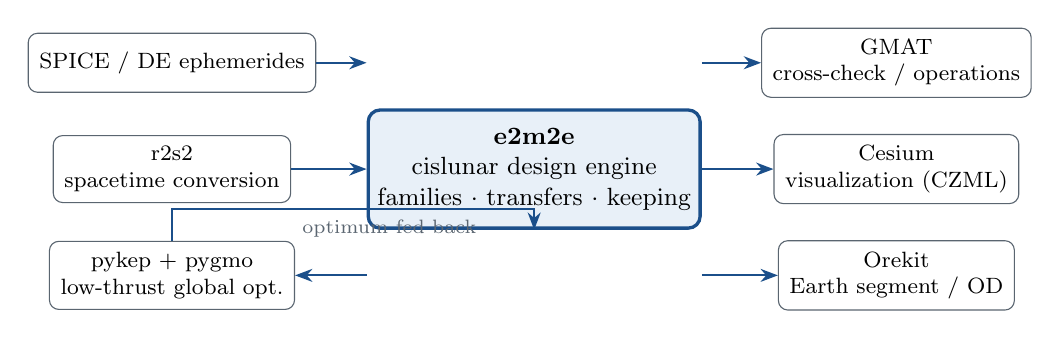
\begin{tikzpicture}[
  font=\footnotesize,
  box/.style={draw=e2gray, rounded corners=1.2mm, fill=white,
    minimum height=0.75cm, align=center, inner sep=4pt},
  core/.style={draw=e2blue, very thick, rounded corners=1.5mm, fill=e2light,
    minimum height=1.5cm, minimum width=3.6cm, align=center, font=\small},
  arr/.style={-{Stealth[length=2.2mm]}, thick, e2blue},
]
\node[core] (e2) at (0,0) {\textbf{e2m2e}\\cislunar design engine\\families $\cdot$ transfers $\cdot$ keeping};
\node[box] (spice) at (-4.6,1.35) {SPICE / DE ephemerides};
\node[box] (r2s2) at (-4.6,0) {r2s2\\spacetime conversion};
\node[box] (gmat2) at (4.6,1.35) {GMAT\\cross-check / operations};
\node[box] (cesium) at (4.6,0) {Cesium\\visualization (CZML)};
\node[box] (orekit) at (4.6,-1.35) {Orekit\\Earth segment / OD};
\node[box] (pykep) at (-4.6,-1.35) {pykep + pygmo\\low-thrust global opt.};
\draw[arr] (spice.east) -- (e2.west |- spice);
\draw[arr] (r2s2.east) -- (e2.west |- r2s2);
\draw[arr] (e2.east |- gmat2) -- (gmat2.west);
\draw[arr] (e2.east) -- (cesium.west);
\draw[arr] (e2.east |- orekit) -- (orekit.west);
\draw[arr] (e2.west |- pykep) -- (pykep.east);
\draw[arr] (pykep.north) -- ++(0,0.4) -| (e2.south) node[pos=0.3, below, font=\scriptsize, text=e2gray] {optimum fed back};
\end{tikzpicture}
\caption{The composition ecosystem of e2m2e: spacetime/ephemeris suppliers
upstream; rendering, cross-checking, orbit determination, and global
optimization consumers downstream---e2m2e holds exactly the cislunar design
engine layer.}
\label{fig:eco}
\end{figure}

\begin{keybox}{Summary: A Repeatedly Verified Vacancy}
The general platforms have no three-body kernel (GMAT), or a framework
without automation (STK/Astrogator), or components without a pipeline
(Orekit), or dynamics without design tools (pykep), while the teaching
library was archived with its three-body work still in contrib drafts
(poliastro)---none of the eight subjects combines ``eight-family generation
+ manifold low-energy transfer + three-body keeping + ephemeris correction
chain''. This vacancy, verified subject-by-subject at the code level, is
e2m2e's niche.
\end{keybox}

\section{Verification and Conclusion}
\label{sec:verification}

\subsection{Verification by Definition}

e2m2e's verification philosophy is \emph{verification by definition}
(ADR 0013): assertions land mainly on analytic solutions, conserved
quantities, and literature formulas, rather than on regression comparisons
``consistent with its own previous output''. The test suite is divided into
six categories by verification target, with directories mirroring the source
layout:

\begin{itemize}
  \item \texttt{algorithm}: orchestration chains of coordinates, dynamics,
        design, correction, and transfer;
  \item \texttt{api}: Facade and MCP interface responses and error
        translation;
  \item \texttt{data}: the data layer---kernels, reference frames, physical
        constants;
  \item \texttt{mbse}: MBSE data models, requirement registration, and
        diagram generation;
  \item \texttt{numerical}: integrator accuracy against analytic orbits;
        force-model accelerations and Jacobians;
  \item \texttt{tools}: auxiliary utilities---logging, formatting,
        visualization.
\end{itemize}

The coordinate and time chains are additionally cross-compared against GMAT
reference data; Rust-side numerical methods are verified against analytic
solutions in \texttt{crates/*/tests/}. High-fidelity propagation accuracy
aligns with GMAT and DFH to the sub-100\,m level. The Lambert solver is
verified against Vallado's classic test case; multi-impulse optimization
reproduces the LEO$\to$GEO Hohmann benchmark of 3.7708 km/s; differential
correction, continuation, and stability analysis are checked against formulas
from Broucke, Richardson, G\'omez, and others.

\subsection{Conclusion and Outlook}

e2m2e converges the complete chain of cislunar mission orbit design---the
spacetime reference, multi-fidelity dynamics, periodic orbit family
generation, three classes of transfer design, and station-keeping
simulation---under a single task-level Facade, guarantees the performance and
parallel safety of heavy iteration with a Rust numerical kernel, and opens
the entire chain to LLM agents through the MCP interface. It does not pursue
the full coverage of general-purpose tools; instead, in the sufficiently deep
domain of cislunar space, it makes every step from initial guess to
verification a composable, traceable, and auditable engineering component.

On the roadmap: the unified ephemeris-serialization intermediate format
EphemerisTable with converters to/from CCSDS OEM/ODM, SPICE BSP/PCK, and
other typical formats; further migration of remaining Python numerics (such
as NLP optimization) into the Rust kernel; and, building on the orbit catalog
as a data foundation, extensions toward intelligent game-theoretic research.

\begin{center}
\small
\begin{tabular}{@{}ll@{}}
\toprule
\textbf{Repository} & \url{https://github.com/cislunarspace/e2m2e} \\
\textbf{Documentation} & \url{https://cislunarspace.github.io/e2m2e/} \\
\textbf{License} & Apache 2.0 \\
\textbf{Install} & \texttt{uv pip install e2m2e} \\
\bottomrule
\end{tabular}
\end{center}


\end{document}
